\section{INTRODUCTION}

This document serves as formal documentation of the implementation of
the \textit{rnucs} tally in MCNP6.2. A comparison to the implemention
in MCNP6.1 will be shown in this document. 

\section{COMPARISON OF RNUCS IN MCNP6.1 AND MCNP6.2}

\subsection{Geometry}
A simple geometry was selected and can be seen in Figure \ref{fig:merbox.png}.
A Gaussian distribution centered around 1GeV proton source was used. 
The source is located in the xy plane at z = -256.71 cm, where the x position is
dependent in the y position. 


\begin{figure}[h!]
        \centering
        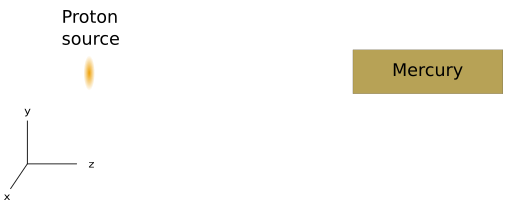
\includegraphics[scale=0.7]{figs/mercury.png}
        \caption[VPI]{Planar view of the testing geometry}
        \label{fig:merbox.png}
\end{figure}


\subsection{MCNP Transport}
A transport calculation was performed using MCNP6.1 and MCNP6.2.
1E8 particles, and the geomtry previously presented. 
The isotope production and destruction in the mercury volume was collected
using the rnucs tally. 
Figures \ref{fig:prod} and \ref{fig:dest}  show the isotope production
and isotope destruction collected in the mercury volume. These figures also
show the relative difference between the results collected in MCNP6.1
and MCNP6.2. 
The relative difference is given by the following equation:
\begin{equation}
	\frac{MCNP6.2 - MCNP6.1}{MCNP6.1}.
\end{equation}


\begin{figure}[h!]
        \centering
        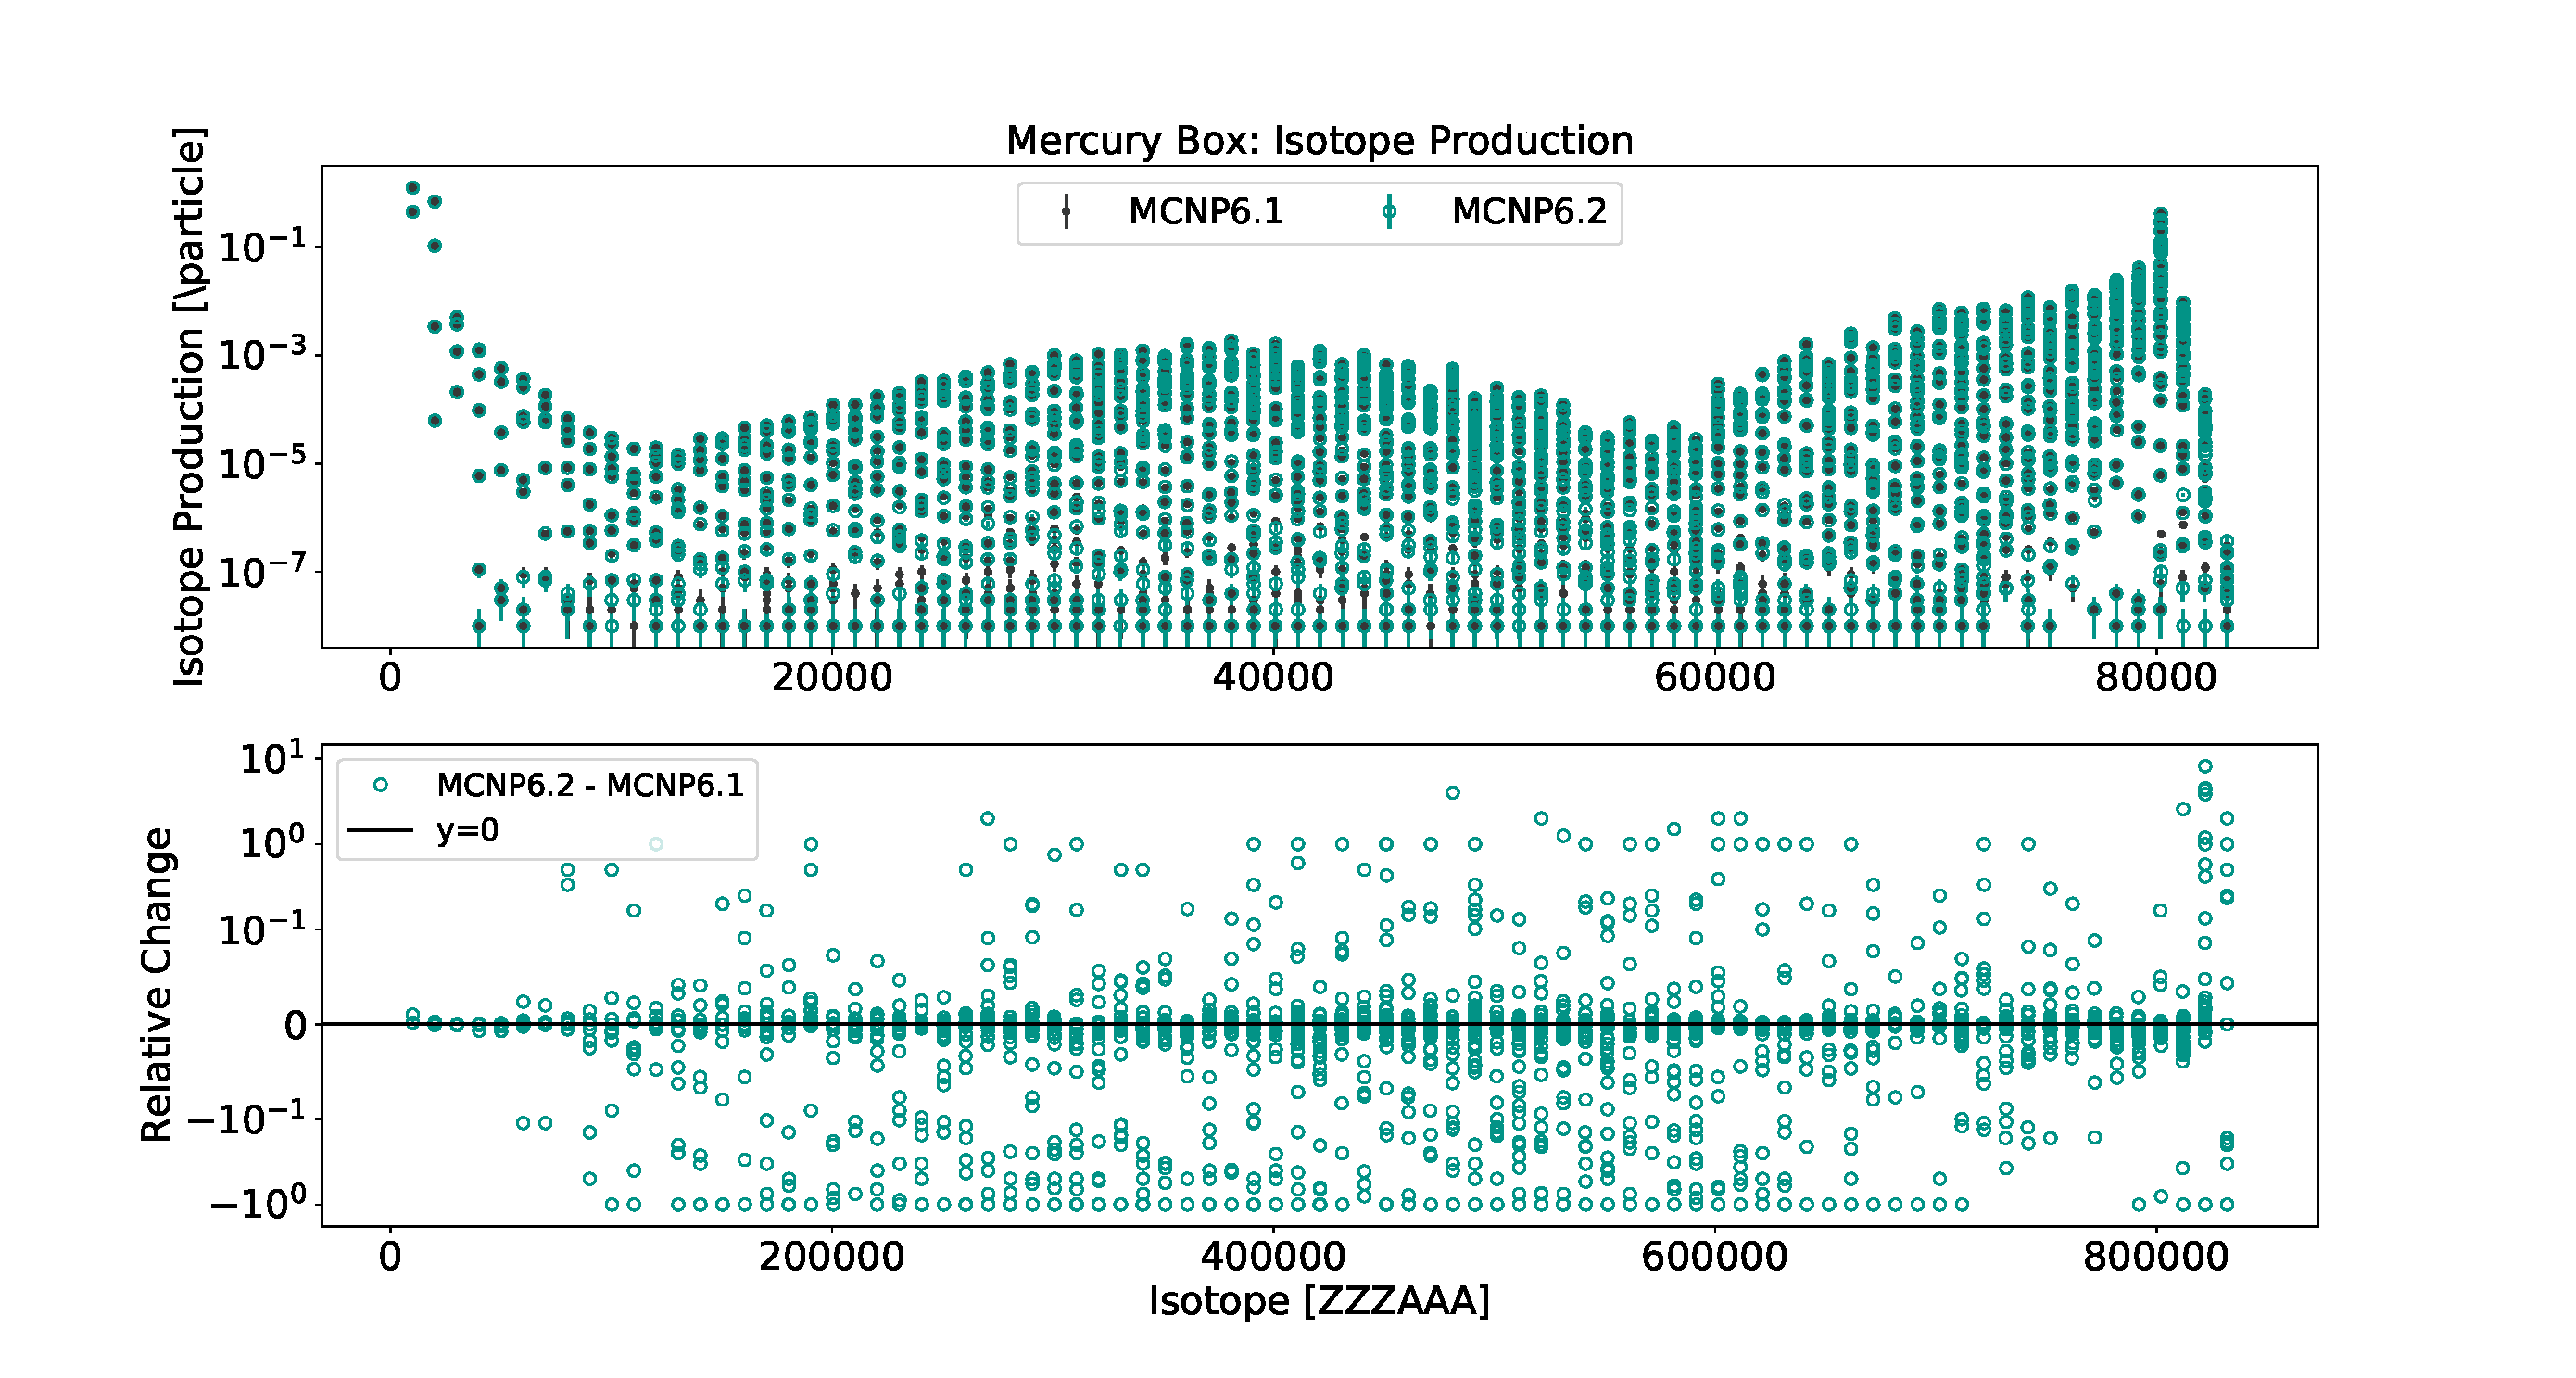
\includegraphics[scale=0.4]{figs/prod_merbox_62_61.pdf}
	\caption{Isotope Production in the Mercury volume}
        \label{fig:prod}
\end{figure}

\begin{figure}[h!]
        \centering
        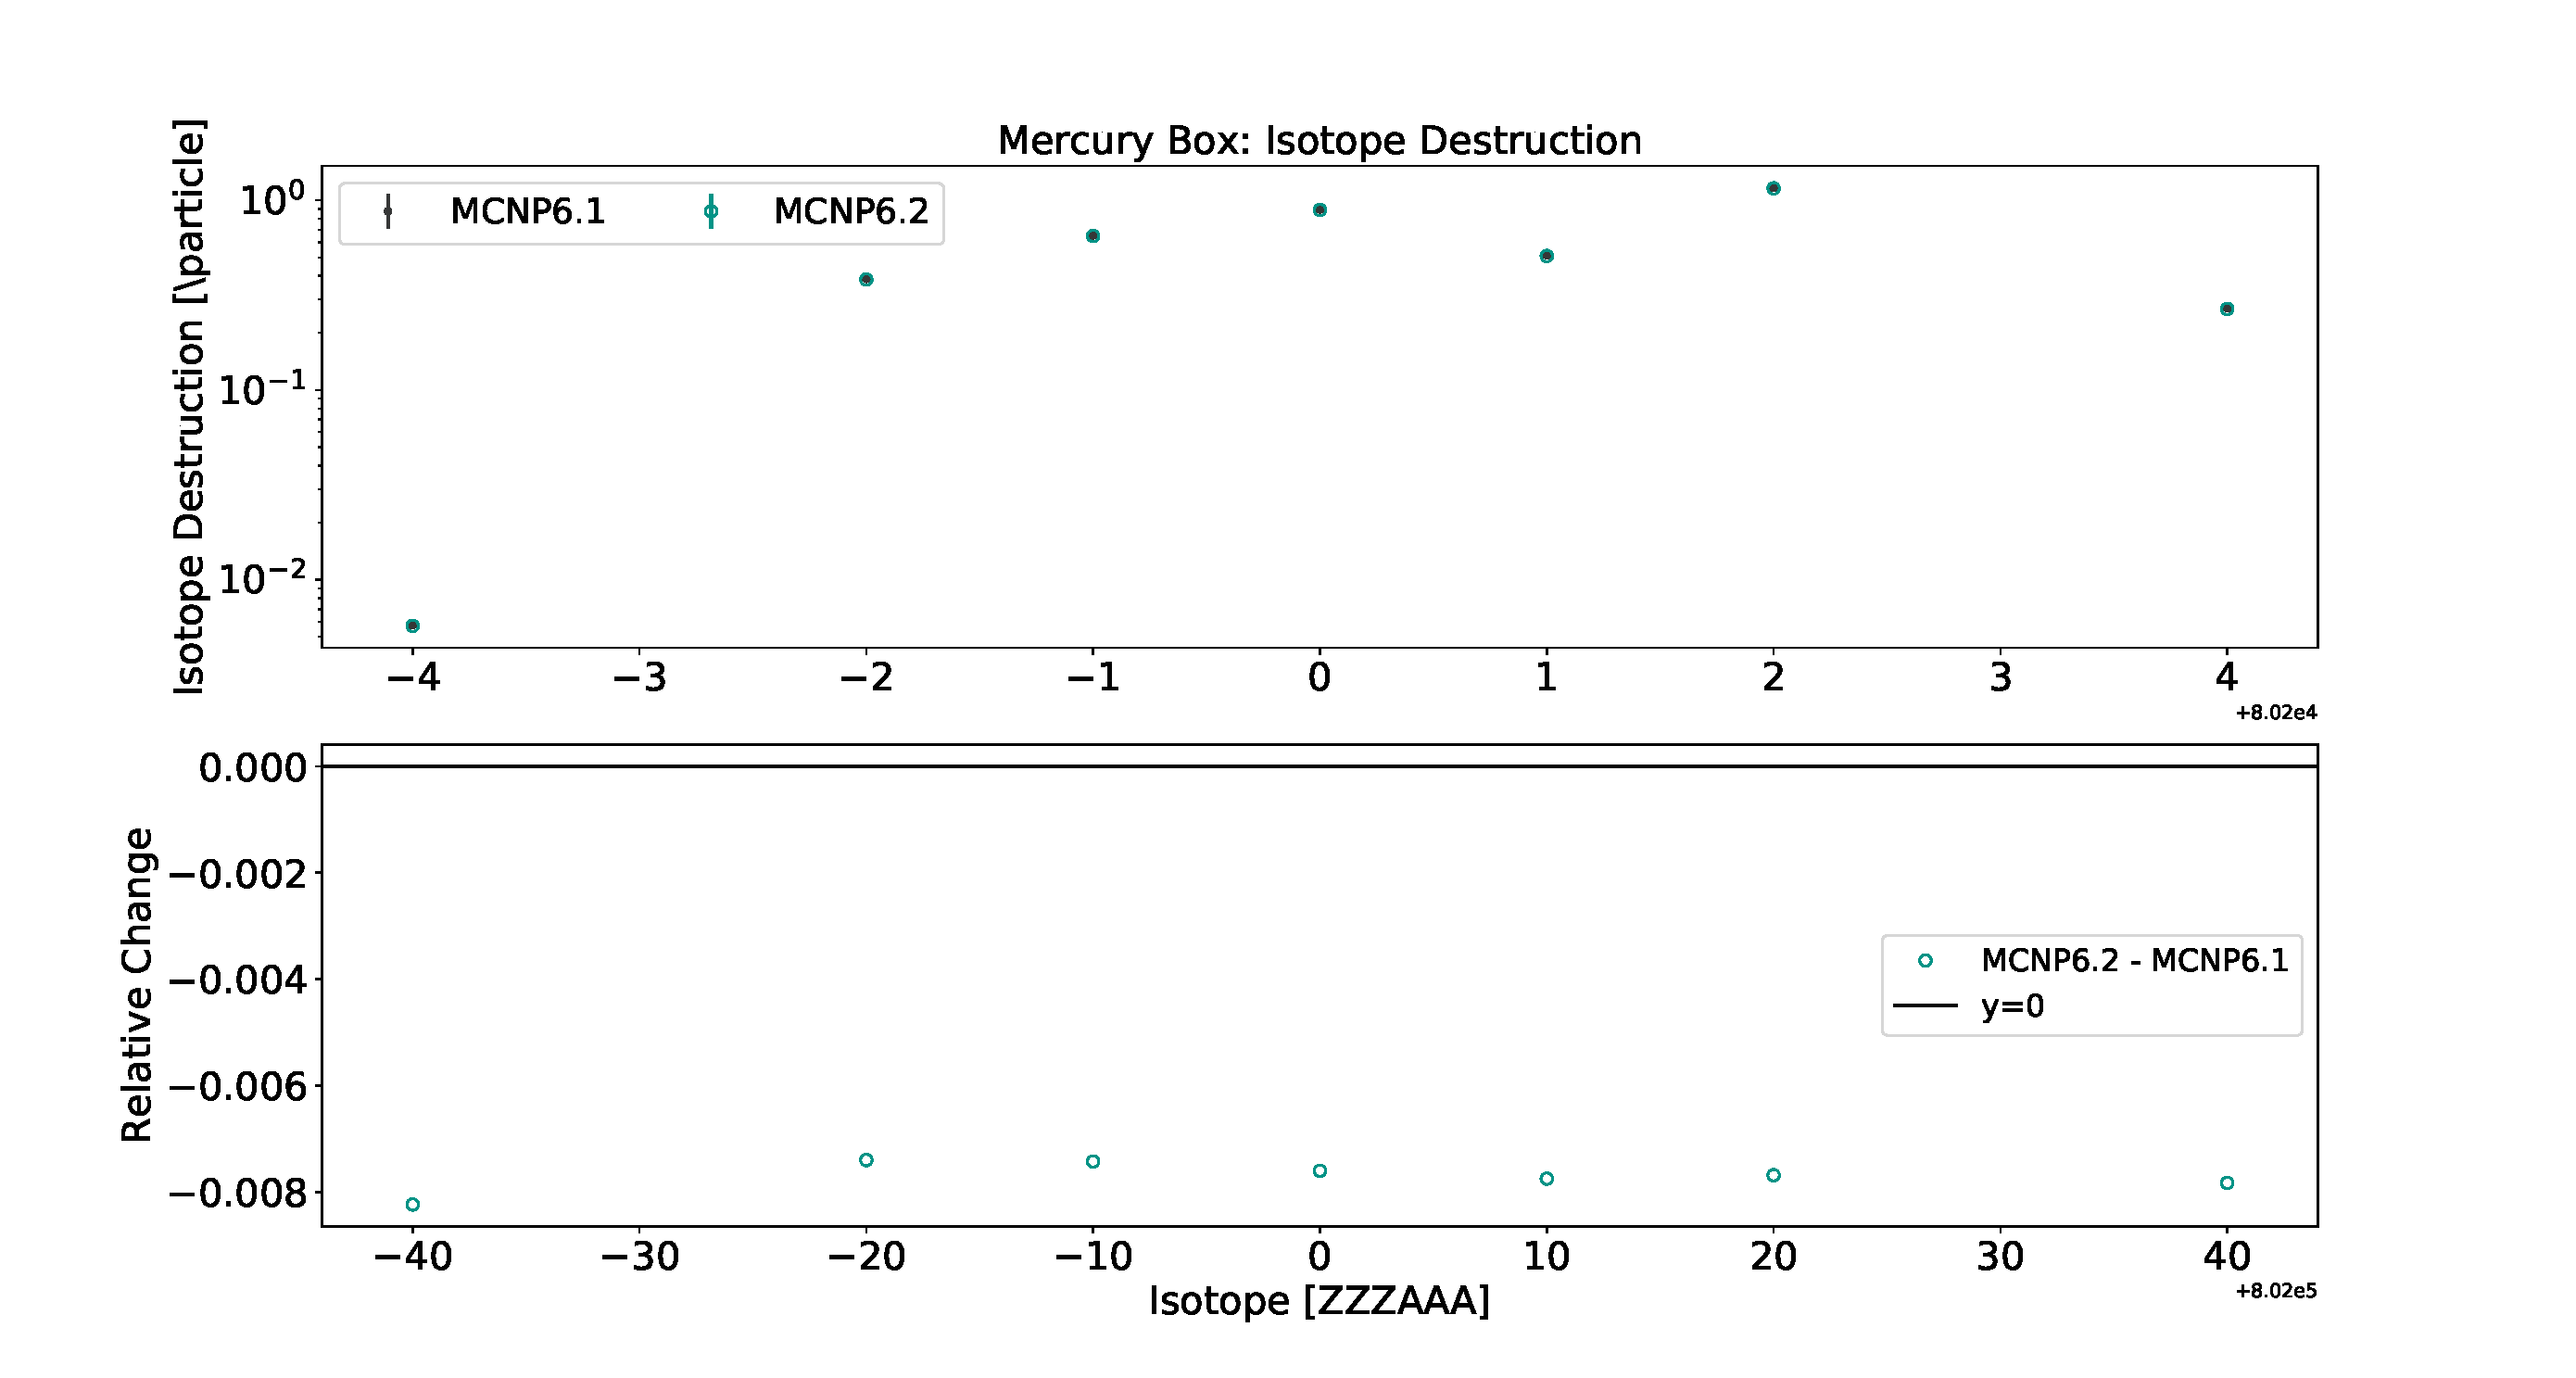
\includegraphics[scale=0.4]{figs/dest_merbox_62_61.pdf}
	\caption{Isotope Destruction in the Mercury volume}
        \label{fig:dest}
\end{figure}

Figure \ref{fig:prod} shows a more significant difference than those in
Figure \ref{fig:dest}. In order to better understand the importance of
the difference, a graph representing the relative difference versus the
isotope production data is shown in Figure \ref{fig:reldiff}. This 
figure shows a correlation between the high relative difference and
low isotope production.

\begin{figure}[h!]
        \centering
        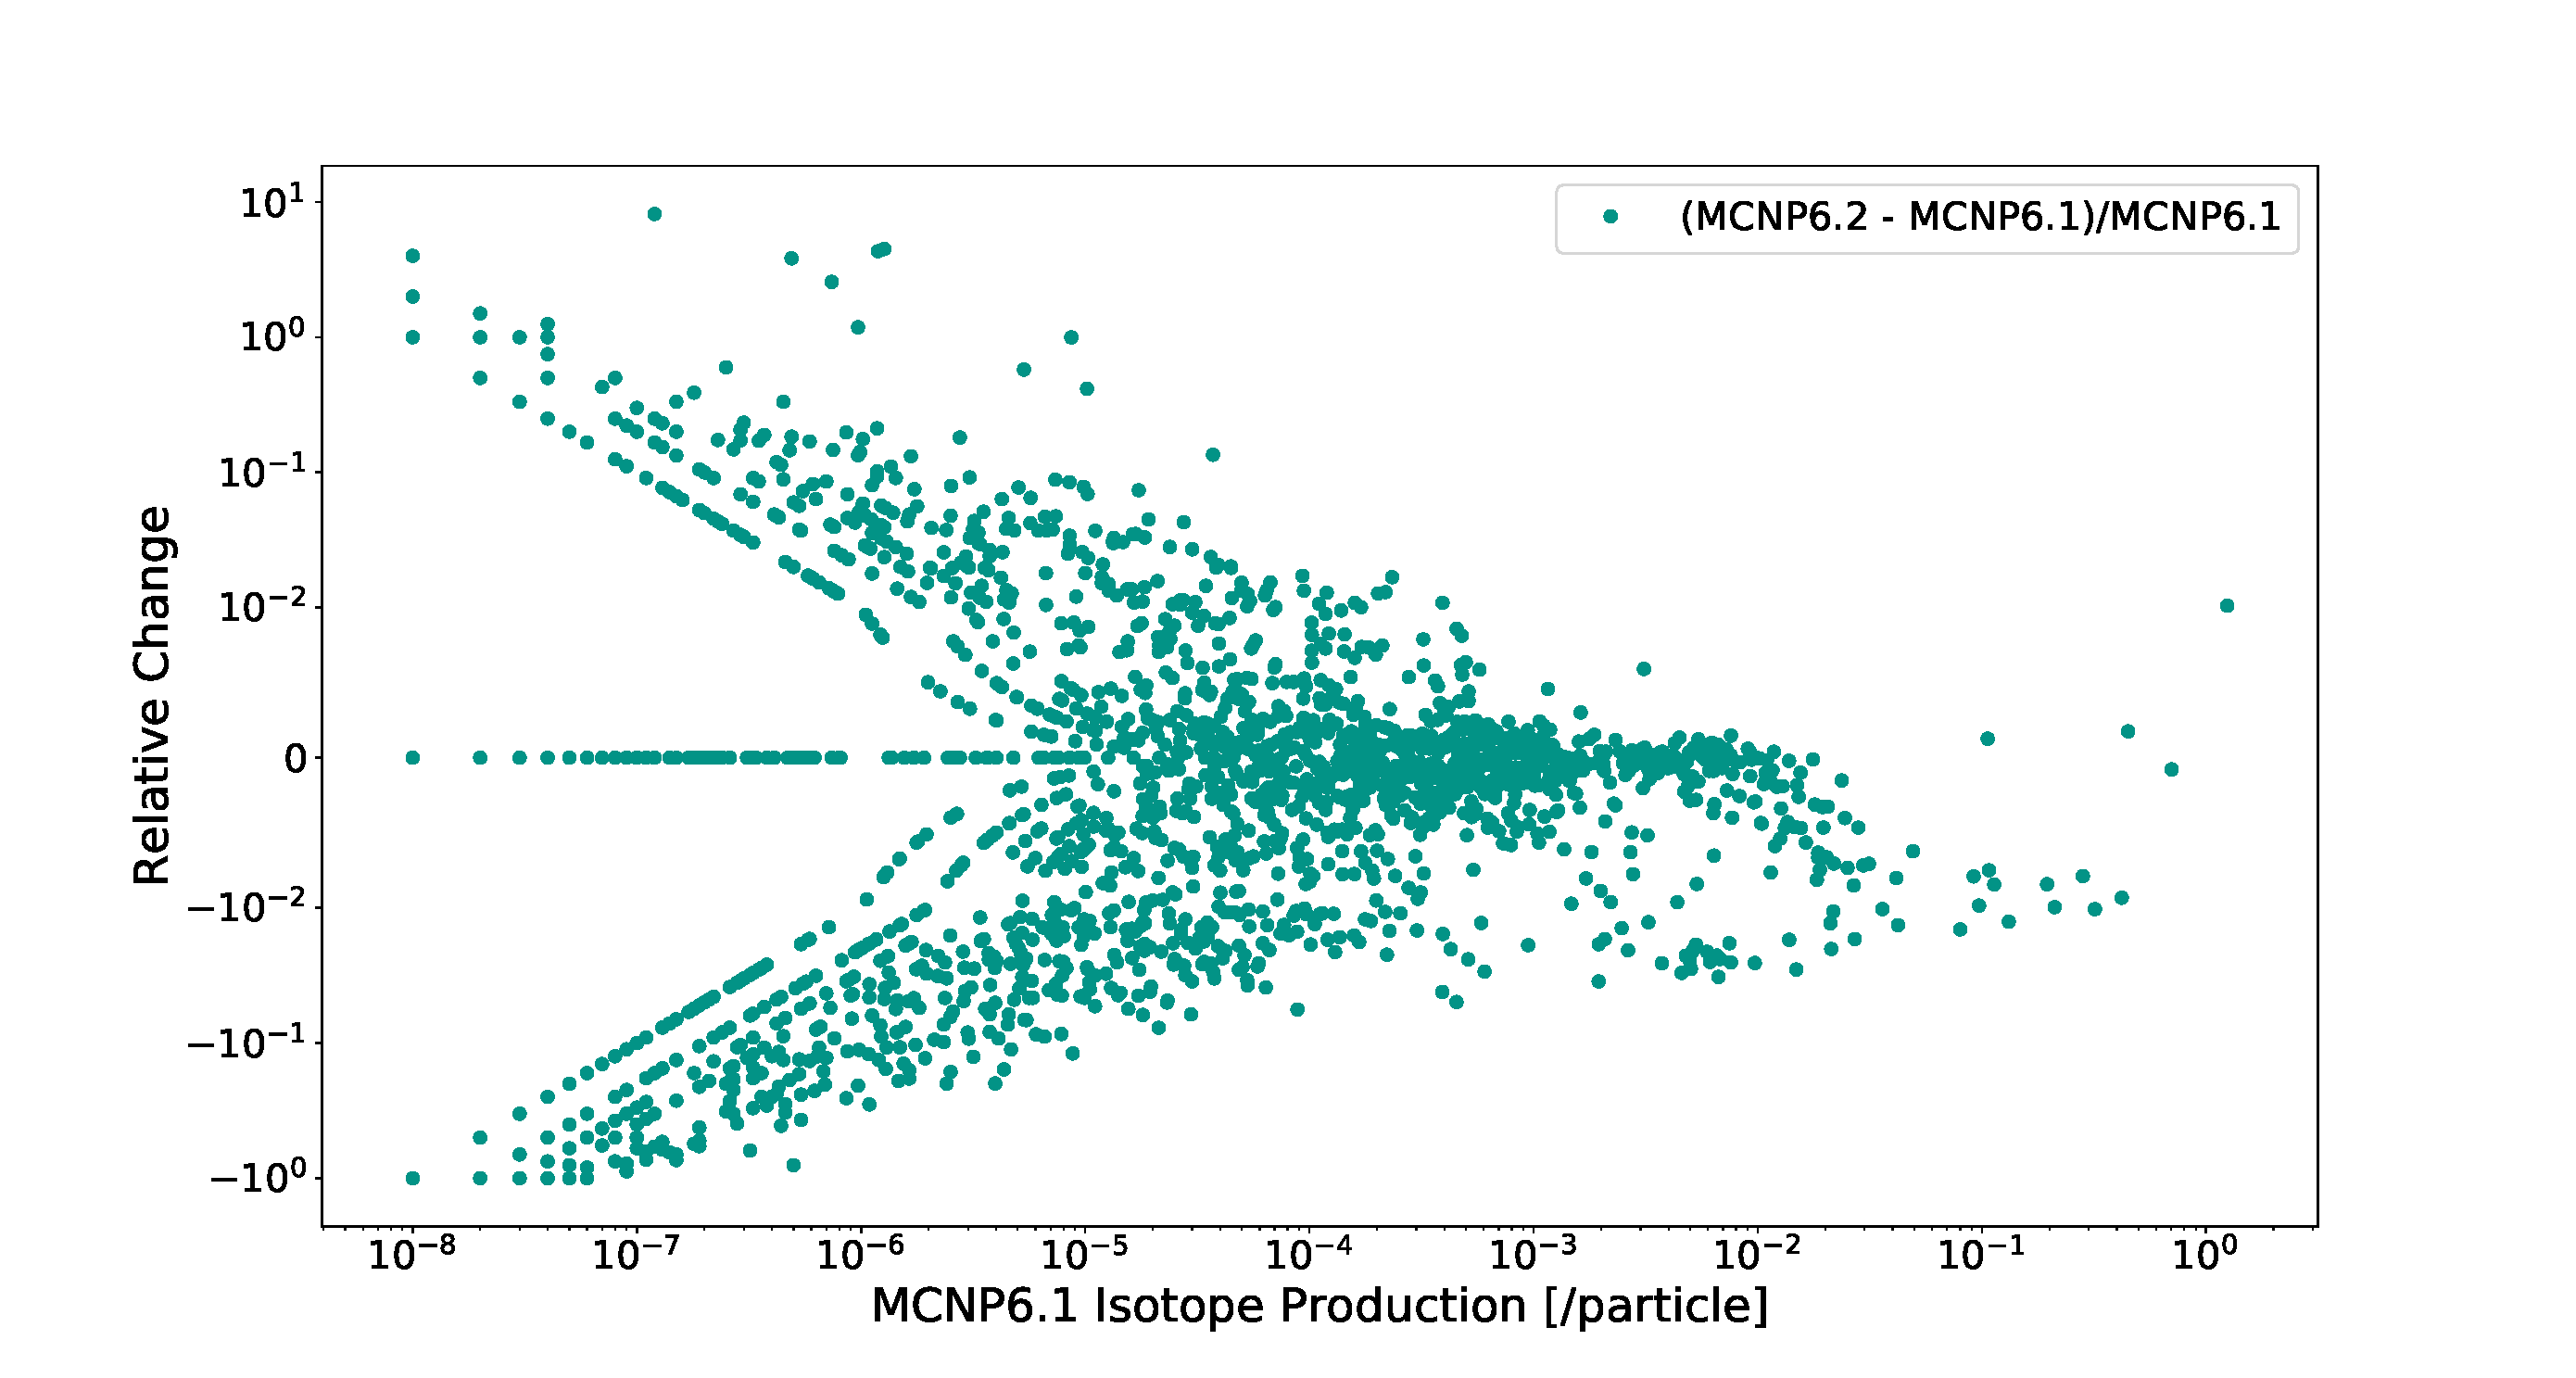
\includegraphics[scale=0.4]{figs/reldiff_merbox_62_61.pdf}
	\caption{Relative Difference vs. Isotope Production}
        \label{fig:reldiff}
\end{figure}

Another metric used to compare the results is the Z-Score. A Z-score
is a quantity that tells us how many sigmas a value is from a population
mean. For this comparison, two sample means are compare and the following
equation was used. 
\begin{equation}
        z = \frac{\bar{x} - \mu }{\sigma / \sqrt{n}}
\end{equation}
where
\begin{equation}
\begin{split}
        \bar{x} &= \text{Sample mean} \\
        \mu     &= \text{Population mean} \\
        \sigma  &= \text{Population standard deviation} \\
        n       &= \text{Sample size}
\end{split}
\end{equation}

